\chapter{Implementation}

\section{Parsers}

\subsection{Recursive Descent Parser}

The first \href{https://github.com/ElektraInitiative/libelektra/commit/3d2d4644cb08e83f0b3305b8aeae546ada52dfe7}{\glstext{YAML} plugin} we developed used a handwritten recursive descent parser. As already described in “\nameref{sec:state_of_the_art}” this technique is quite popular, since there exists a natural correspondence between code and grammar rules. Table~\ref{tab:recursive_descent_correspondence} shows the correspondence between \gls{ABNF} grammar rules and matching C like pseudo-code.

\begin{table}[H]
  \begin{center}
    \begin{tabular}{llp{0.48\textwidth}}
      \toprule
      Grammar & Example & Code\\
      \midrule

      \vspace{0cm}
      Terminal
      &
      \vspace{0cm}
      \codebox{
      \texttt{{\color{color02} a}
              {\color{color03} \textbf{=}}
              {\color{color07} "a"}}}
      &
      \vspace{-0.36cm}
      \begin{minted}[autogobble]{c}
        bool a() {
          bool match = getc(file) == 'a';
          if (!match) putc(file);
          return match;
        }
      \end{minted}
      \\

      \vspace{0cm}
      Sequence
      &
      \vspace{0cm}
      \codebox{
      \texttt{{\color{color02} seq}
              {\color{color03} \textbf{=}}
              {\color{color02} rule1 rule2}}}
      &
      \vspace{-0.36cm}
      \begin{minted}[autogobble]{c}
        bool seq() {
          return rule1() && rule2();
        }
      \end{minted}
      \\

      \vspace{0cm}
      Alternative
      &
      \vspace{0cm}
      \codebox{
      \texttt{{\color{color02} seq}
              {\color{color03} \textbf{=}}
              {\color{color02} rule1}
              {\color{color03} /}
              {\color{color02} rule2}}}
      &
      \vspace{-0.36cm}
      \begin{minted}[autogobble]{c}
        bool alt() {
          return rule1() || rule2();
        }
      \end{minted}
      \\

      \bottomrule
    \end{tabular}
  \end{center}
  \caption{Correspondence between grammar rules and code in a recursive descent parser}
  \label{tab:recursive_descent_correspondence}
\end{table}

\newpage
While Table~\ref{tab:recursive_descent_correspondence} suggest writing a recursive descent parser is trivial, there are many problems that the code above does not take into account:

\begin{description}
  \item [Recognizer Only:] The pseudo-code only implements a recognizer for the language. At the end of the parsing process we only know, if the input is part of the language produced by the given grammar or not. Usually we want to \emph{build a data structure}, in our case a \cc{KeySet}, from the given input.

  \item [Error Handling:] The code does not contain any error handling. If a given input contains errors, then the author of the \glstext{YAML} data wants to know \emph{where these errors occurred}. Otherwise she or he has to check the whole input.

  \item [Left Recursion:] If we translate a left recursive rules such as \code{\color{color02} rule1 \color{color03} \textbf{=} \color{color02} rule1 \color{color03} / \color{color02} rule2} using the correspondences given in Table~\ref{tab:recursive_descent_correspondence}, then the resulting code would never terminate. This is the case, since \code{\color{color02} rule1} calls \code{{\color{color02} rule1}}, which then calls \code{\color{color02} rule1}, and so on an so forth (infinite recursion).
\end{description}

All of the problems above apply regardless of the programming language of the parsing code. Since we implemented the recursive descent parser in C, another issue is the error handling in C itself. The language does not provide a native exception handling mechanism. We therefore used the return value to also transfer the error information between functions. This approach is quite cumbersome, since it basically means that we have to check for an error after each function call.

We used C macros to minimize the code overhead and complexity caused by the error handling. Still, for a very small part of the \glstext{YAML} syntax described in the ABNF grammar of Figure~\ref{cod:abnf_recurive_descent} the parser contained about 374 lines of code (counted with \code{cloc} version 1.72). While smaller feature additions, such as going from support of one key-value pair to multiple key-value pairs \href{https://github.com/ElektraInitiative/libelektra/commit/17aa7a6ea5d9261287104213dcba67f4d0a0fcbc}{were quite straightforward} (\textcolor{Green}{14 additions}, \textcolor{Red}{1 deletion}), other modifications, such as supporting block styles would take considerable more effort.

Since the first steps with a hand-written recursive descent parser showed that this approach takes considerable effort we decided against extending the first prototype. Instead we chose to use an already existing hand-written \glstext{YAML} parser.

\begin{listing}
  \centering
  \begin{code-boxed}
    {\small
{\color{color02} NEL} {\color{color03} \textbf{=}} {\color{color04} \%x85}{\color{color05} \\}{\color{color02} WSLF}
{\color{color03} \textbf{=}} {\color{color04} \textbf{WSP}} {\color{color03} \textbf{/}}
{\color{color04} \textbf{LF}}{\color{color05} \\\\}{\color{color06} ; Printable
characters from C0 set\\}{\color{color02} printable} {\color{color03} \textbf{=}}
{\color{color04} \textbf{HTAB}} {\color{color03} \textbf{/}} {\color{color04} \textbf{LF}}
{\color{color03} \textbf{/}} {\color{color04} \textbf{CR}}{\color{color05} \\}{\color{color06} ;
Printable ASCII\\}{\color{color02} printable} {\color{color03} \textbf{=/}} {\color{color04} \%x20}{\color{color03} \textbf{-}}{\color{color04} 7e}{\color{color05} \\}{\color{color06} ;
Next Line from C1 set\\}{\color{color02} printable} {\color{color03} \textbf{=/}}
{\color{color02} NEL}{\color{color05} \\}{\color{color06} ; Characters after C1
set -- Surrogate pairs\\}{\color{color02} printable} {\color{color03} \textbf{=/}}
{\color{color04} \%xa0}{\color{color03} \textbf{-}}{\color{color04} d7ff}{\color{color05} \\}{\color{color06} ;
Private use characters -- Replacement character\\}{\color{color02} printable}
{\color{color03} \textbf{=/}} {\color{color04} \%xe00}{\color{color03} \textbf{-}}{\color{color04} fffd}{\color{color05} \\}{\color{color06} ;
All Unicode Character Starting from the Supplementary Multilingual Plain\\}{\color{color02} printable}
{\color{color03} \textbf{=/}} {\color{color04} \%x10000}{\color{color03} \textbf{-}}{\color{color04} 10ffff}{\color{color05} \\\\}{\color{color02} pairs}
{\color{color03} \textbf{=}} {\color{color03} \textbf{*}}{\color{color02} WSLF}
{\color{color07} \texttt{"}\{\texttt{"}} {\color{color02} pair} {\color{color02} optionalAdditionalPairs}
{\color{color07} \texttt{"}\}\texttt{"}} {\color{color03} \textbf{*}}{\color{color02} WSLF}{\color{color05} \\}{\color{color02} optionalAdditionalPairs}
{\color{color03} \textbf{=}} {\color{color03} \textbf{*(}}{\color{color07} \texttt{"},\texttt{"}}
{\color{color02} pair}{\color{color03} \textbf{)}}{\color{color05} \\}{\color{color02} pair}
{\color{color03} \textbf{=}} {\color{color02} key} {\color{color07} \texttt{"}:\texttt{"}}
{\color{color02} value}{\color{color05} \\}{\color{color02} key} {\color{color03} \textbf{=}}
{\color{color02} doubleQuotedSpace}{\color{color05} \\}{\color{color02} value}
{\color{color03} \textbf{=}} {\color{color02} doubleQuotedSpace}{\color{color05} \\}{\color{color02} doubleQuotedSpace}
{\color{color03} \textbf{=}} {\color{color03} \textbf{*}}{\color{color02} WSLF}
{\color{color02} doubleQuoted} {\color{color03} \textbf{*}}{\color{color02} WSLF}{\color{color05} \\}{\color{color02} doubleQuoted}
{\color{color03} \textbf{=}} {\color{color04} \textbf{DQUOTE}} {\color{color02} content}
{\color{color04} \textbf{DQUOTE}}{\color{color05} \\}{\color{color02} content}
{\color{color03} \textbf{=}} {\color{color03} \textbf{*}}{\color{color02} printable}
}

  \end{code-boxed}
  \caption{ABNF grammar for a very small regular subset of \glstext{YAML}}
  \label{cod:abnf_recurive_descent}
\end{listing}

The official \href{http://yaml.org}{YAML website} prominently lists known \glstext{YAML} parsers. Since we decided to use C or C++ as programming language – to improve the comparability of the parsers – we are left with three basic options:

\begin{itemize}
  \item Syck (\glstext{YAML} 1.0)
  \item \href{https://github.com/yaml/libyaml}{LibYAML} (YAML 1.1)
  \item \href{https://github.com/jbeder/yaml-cpp}{yaml-cpp} (YAML 1.2)
\end{itemize}

. Out of these options Syck is not actively maintained any more. This leaves only \code{libyaml} and \code{yaml-cpp}. We decided to use \code{yaml-cpp}, since it supports the latest version of \glstext{YAML} (\code{YAML 1.2}). With the help of the library we \href{https://github.com/ElektraInitiative/libelektra/pull/1613}{added the first plugin with full YAML support} called \href{https://www.libelektra.org/plugins/yamlcpp}{YAML CPP} to Elektra.

\subsection{ALL(*) Parser}

The first parser generator we used as part of the thesis was \gls{ANTLR} 4. As we already described in the section “\nameref{sec:state_of_the_art}” ANTLR 4 generates parsing code that uses an adaptive LL algorithm called ALL(*). As target language for the generated parser we used the \href{https://github.com/antlr/antlr4/pull/1210}{C++ target for ANTLR}, which was added to the official repository of ANTLR 4 in 2016.

\subsubsection{Initial Attempt}

One of the first problems we encountered using ANTLR was the significant leading whitespace used to describe the structure of \glstext{YAML} block \glspl{collection}. In \glstext{YAML} increased leading whitespace starts a new child element, while decreasing amount of leading whitespace ends an element. Users of programing languages such as \href{https://www.python.org}{Python} or \href{https://www.haskell.org}{Haskell} should be familiar with this style. Unlike \href{https://docs.python.org/3/reference/grammar.html}{Python’s grammar}, \glstext{YAML}’s reference grammar does not use \code{INDENT} and \code{DETEND} tokens, but uses parameterized \gls{BNF} productions instead. According to the authors of the \glstext{YAML} specification, this is necessary to describe the indentation rules of \glstext{YAML}~\cite{ben2009yaml}:

\begin{quote}
  Many productions use an explicit indentation level parameter. This is less elegant than Python’s “indent” and “undent” conceptual tokens. However it is required to formally express \glstext{YAML}’s indentation rules.
\end{quote}

. We first tried to parse different levels of whitespace using \href{https://github.com/sanssecours/Yan-LR/compare/0b0deae...7d9e64e}{\emph{semantic predicates} and \emph{rule arguments}}~\cite{parr1995antlr}. Semantic predicates allow us to disable certain parts of a grammar dynamically, while we can use rule arguments to specify different amount of whitespace. This approach worked, but only for a constant amount of whitespace. If we tried to specify a different amount of leading spaces in a grammar rule, dependent on the amount of leading whitespace matched in the current rule, then the generated parser would be unable to parse simple example input.

\subsubsection{Indent \& Detend Tokens}

Since the initial attempt for our ANTLR grammar did not show promising results, we looked at how other ANTLR grammars handle significant whitespace.

Bart Kiers created an \href{https://github.com/antlr/grammars-v4/blob/master/python3/Python3.g4}{ANTLR grammar for Python 3}, which captures the start of a document and newline characters inside the lexer. The grammar then uses application-specific code~\cite[p. 48]{parr2013definitive} to fill a stack with the current amount of indentation and emits \code{INDENT} and \code{DETEND} tokens accordingly. Since this method looked promising, we created a \href{https://github.com/sanssecours/Yan-LR/compare/363be1e...188e5d4}{basic \glstext{YAML} parser that used the same algorithm}. While this approach worked for some \glstext{YAML} documents, we found simple input where the algorithm did not show the expected result. Another problem with this approach are complex lexer rules for \glstext{YAML} scalars. The cause of this problem is that the parameterized BNF rules of the \glstext{YAML} specification do not translate well to the basic lexer syntax used to specify characters and character ranges provided by ANTLR.

\subsubsection{Custom Lexer}

For the \href{https://www.libelektra.org/plugins/yanlr}{final version of our ANTLR parser} we looked at the source code of various \glstext{YAML} parsing libraries. One of the most widely used parsing libraries is \href{https://github.com/yaml/libyaml}{LibYAML}. LibYAML is especially interesting since it was implemented by Kirill Simonov under the guidance of one of the authors of the \glstext{YAML} specification: Clark Evans~\cite{libyaml2018pyyaml}.

Unfortunately LibYAML’s code uses C macros quite heavily and is therefore not very readable. A quick look at the code and comments showed us that LibYAML’s handwritten lexer already takes care of issues such as proper detection of plain scalars and \glspl{simpleKey}. Since the lexer uses a turing-complete language to scan the input, it is also able to handle nested block \glspl{collection}.

The source code of LibYAML showed us that we can take care of most of \glstext{YAML}’s  complexity in the lexer. For further information we looked at \href{https://github.com/llvm/llvm-project/blob/master/llvm/lib/Support/YAMLParser.cpp}{LLVM’s YAML parser} (written in C++) and \href{https://bitbucket.org/asomov/snakeyaml-engine}{SnakeYAML Engine} (written in Java). The lexer of both of these tools use the same basic ideas as LibYAML. However, the code of these libraries is easier to read than LibYAML’s, since LLVM’s YAML parser and SnakeYAML Engine are written in higher level programming languages.

The most interesting part in the lexer of the libraries described above, is probably how they are able to add tokens for \glspl{simpleKey}. The text below describes how the algorithm works (in SnakeYAML Engine).

\begin{itemize}

  \item The lexer keeps a list of tokens and stores how many of those token it has emitted. The lexer can not simply emit a token unconditionally, since it might have to scan additional tokens to check if the current token starts a \gls{simpleKey}.

  \item When the lexer scans a \glstext{YAML} token that can possibly start a simple key at the current position it adds this token as simple key candidate. For each simple key candidate the lexer also stores the current position in the token list. This way it can insert a key token at this position later, if a key candidate does indeed start a mapping key.

  \item The lexer only emits the current token, if there are currently no candidates for simple keys. If there are simple key candidates it scans further ahead. Later it

  \begin{enumerate}
    \item removes simple key candidates if the current lexer position is more than 1024 characters ahead of the start position of the key candidate, or if the key candidate does not start in the current line.

    \item adds a key token for a candidate, if it locates a key value symbol (\yaml{:}) for the key candidate.
  \end{enumerate}

\end{itemize}

We used the algorithm described above in the final version of our basic ANTLR storage plugin \href{https://www.libelektra.org/plugins/yanlr}{Yan LR}. For that purpose we wrote a custom \glstext{YAML} lexer. Since the lexer takes care of most of the work, the \href{https://github.com/ElektraInitiative/libelektra/blob/48ccea7107584b1aa28f19ab2b65c9b30090f124/src/plugins/yanlr/YAML.g4}{YAML subset grammar} itself is quite simple, spanning about 30 lines.

\subsection{LALR(1) Parser}

After we finished the initial version of the ANTLR plugin \href{https://www.libelektra.org/plugins/yanlr}{Yan LR} we developed a C++ plugin, that uses a \href{https://www.gnu.org/software/bison}{Bison} parser, called \href{https://www.libelektra.org/plugins/yambi}{YAMBi}.

For the lexer of the plugin we used a slightly modified version of Yan LR’s lexer. This was necessary since Bison, unlike ANTLR, does not provide helper methods to operate on a character stream. For that purpose we wrote a simple class that mimics the behavior of ANTLR’s \cpp{ANTLRInputStream}.

Apart from the parsing algorithm, another difference between Yan LR and YAMBi is the approach on how the plugin translates \glstext{YAML} data to a \cpp{KeySet}. For YAN LR we use a listener interface that operates on the parse tree created by ANTLR. Bison only offers parser actions. These actions contain code that will be called after the parser matches certain parts of the grammar.

YAMBi uses parser actions to call methods of a class that stores temporary data to create the \cpp{KeySet}. The code for this approach is actually not that different from the one of the listener we use for Yan LR. The only problematic part was translating code that added a \cpp{Key} for a \glstext{YAML} mapping that contains no value to a \cpp{KeySet}. For Yan LR we just check, if the mapping parser rule matched a value. This data is already available when we enter the rule, since the listener operates on a completed parse tree. In the corresponding grammar rule of the Bison parser this information is not available yet. To solve this problem we added an \href{https://git.libelektra.org/blob/0c47d024256d0824577209d95d69876722af6248/src/plugins/yambi/parser.ypp#L63-L66}{additional action} to the Bison grammar and moved the code that adds an empty key into a later phase of the parsing process.

\subsection{Earley Parser}
\label{sec:earley_parser}

For the Earley parser plugin we used a parsing library called \href{https://github.com/vnmakarov/yaep}{\gls{YAEP}}. Unlike ANTLR and Bison, \gls{YAEP} does not generate parsing code, but uses a function to parse input according to a user specified grammar. The output of YAEP is a heterogenous \gls{AST}. To construct the tree the user annotates the grammar with tree construction rules (marked with \code{\#}). For example, the first line in the code:

\begin{shellcode}
elements : element          # 0
         | elements element # elements(0 1)
         ;
\end{shellcode}

states that the rule \code{elements} should return the same node \code{element} produced (\code{0}), if it matches a single \code{element}. If the rule \code{elements} matched a rule \code{elements} followed by the rule \code{element} (second line), then YAEP creates a new node with the name \code{elements} that contains the nodes produced by the rule \code{elements} as first child (\code{0}) and the node produced by \code{element} as second child (\code{1}).

Since the output of our storage plugin \href{https://www.libelektra.org/plugins/yawn}{YAwn} should be a \cc{KeySet} and not an \gls{AST}, we created a function that traverses (“walks”) the \gls{AST}. This function calls certain methods of an auxiliary class \code{Listener} that creates the \cc{KeySet}. We already used this pattern for the ANTLR plugin \href{https://www.libelektra.org/plugins/yanlr}{Yan LR}. The most significant difference to the approach used in Yan LR is, that we had to write the tree walking code ourselves.

\subsection{PEG Parser}
\label{sec:peg_parser}

All of the previously described parser generators and libraries divide the parsing process into two distinct phases:

\begin{enumerate}
  \item lexing (generating a stream of symbols from the textual input), and
  \item parsing (forming a data structure from the stream of symbols emitted by the lexer)
\end{enumerate}

. Figure~\ref{fig:lexing_parsing} shows a graphical example of this process.

\begin{figure}
  \centering
    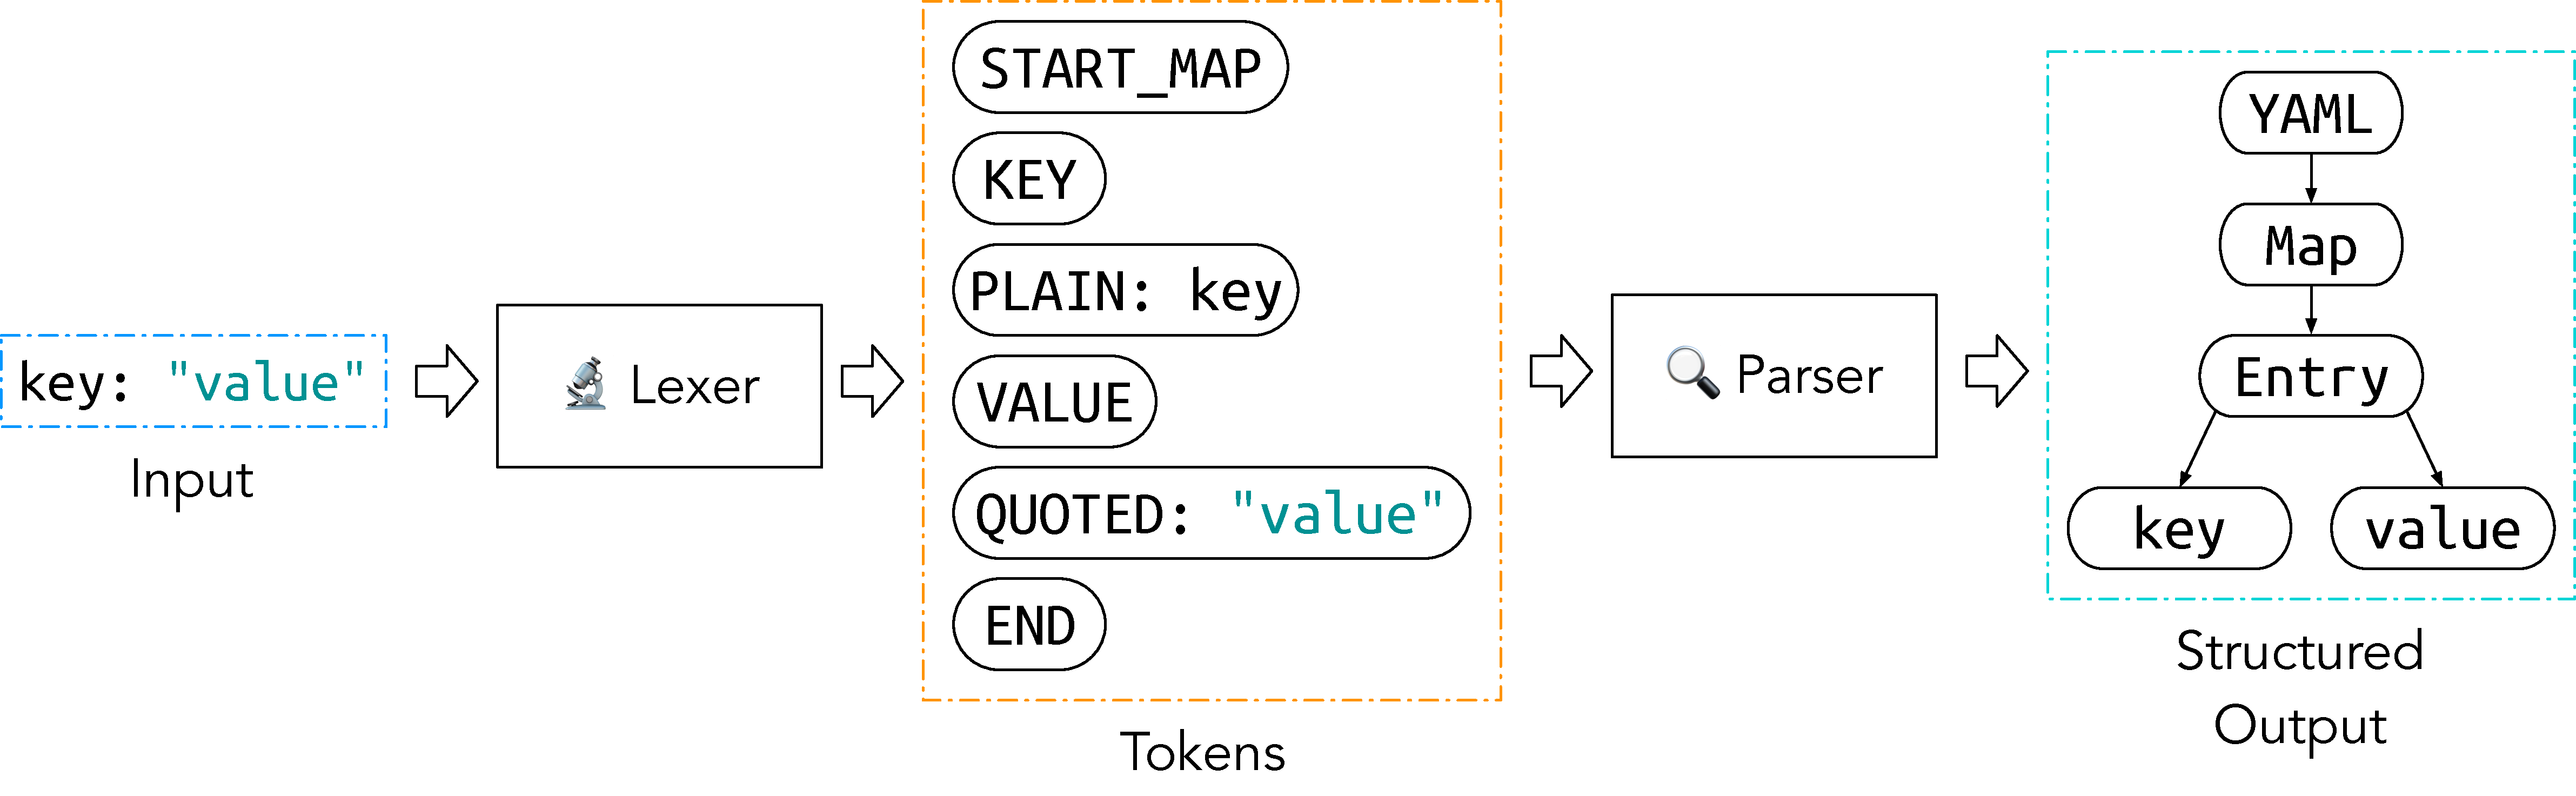
\includegraphics[width=\textwidth]{LexingParsing}
  \caption{A lot of parser engines use two distinct phases (lexing and parsing) to process input}
  \label{fig:lexing_parsing}
\end{figure}

Unlike ANTLR, Bison and YAEP, the library \href{https://github.com/taocpp/PEGTL}{PEGTL} does not use a separate lexing phase. Instead the \gls{PEGTL} parses the input in one sweep using C++ templates to combine simple matching functions into more elaborate parsers. The process of combining parsers this way is also known under the name “parser combinators” (see also Section “\nameref{sec:state_of_the_art}”). Besides the possibility to create \emph{custom matching function}, the library also supports,

\begin{itemize}
  \item \emph{custom actions} to react to matched input, and
  \item \emph{custom state} to store contextual data
\end{itemize}

. Using the three features above we were able to create a \gls{PEG} parser plugin called \href{https://libelektra.org/plugins/yaypeg}{YAy PEG} that uses grammar rules that are similar to the ones described by the \href{http://yaml.org/spec/1.2/spec}{YAML specification}.

The translation of some of the rules from the \glstext{YAML} specification to \gls{PEGTL} rules was trivial. For example, the rule:

\begin{ccode}
ns-plain-first(c) ::= ( ns-char - c-indicator )
                    | ( ( "?" | ":" | "-" )
                        /* Followed by an ns-plain-safe(c)) */ )
\end{ccode}

translates to the following code:

\begin{cppcode}
struct ns_plain_first : sor<seq<not_at<c_indicator>, ns_char>,
                            seq<one<'?', ':', '-'>,
                                at<ns_plain_safe>>> {};
\end{cppcode}

. The rule \cc{sor} represents ordered choice, meaning that it tries to match it’s template arguments:

\begin{enumerate}
  \item \cc{seq<not_at<c_indicator>, ns_char}
  \item \cc{seq<one<'?', ':', '-'>, at<ns_plain_safe>>}
\end{enumerate}

in order. It succeeds if one of the argument matches, or fails if all of them fail. The rule \cc{seq} on the other hand tries to match all its template arguments in sequence and either succeeds, if all of them succeed, or fails, if one of them fails. The rules \cc{at} and \cc{not_at} represents the \gls{PEG} predicates \cc{&} and \cc{!}. The predicate rule \cc{at} (\cc{&}) succeeds, if the current input matches the given input and fails, if it does not. The predicate rule \cc{not_at} behaves exactly opposite. Neither of these predicates consumes any input. The only remaining rule is \cc{one}, which tries to match any of the given characters, \cc{'?'}, \cc{':'} or \cc{'-'} in our example.

While translating the rule \cc{ns-plain-first(c)} was not that hard, other rules that contained nested contextual data such as:

\begin{ccode}
l+block-sequence(n) ::= ( s-indent(n+m) c-l-block-seq-entry(n+m) )+
                        /* For some fixed auto-detected m > 0 */
\end{ccode}

proved more difficult to express in the \gls{PEGTL}. To translate these kind of rules we added a custom state that contains a stack for the indentation (the values \cc{n} and \cc{n+m} above). In the above example a metarule puts the value \cc{n+m} on the stack before the parser tries to match \cc{s-indent(n+m)} and \cc{c-l-block-seq-entry(n+m)} multiple times. Afterwards the metarule removes the last value from the stack leaving the previous value \cc{n}. We called the general metarule that makes this possible \cc{with_updated_state}:

\begin{cppcode}
  template <typename UpdateStateRule,
            typename RevertStateRule,
            typename... Rules>
  struct with_updated_state :
  seq<UpdateStateRule,
      sor<seq<Rules...>,
          seq<RevertStateRule, failure>>,
      RevertStateRule> {};
\end{cppcode}

. As we can see above \cc{with_updated_state} first invokes the rule \cc{UpdateStateRule} to update the state, then it tries to match a sequence of all rules stored in the template parameter pack \cc{Rules}. Depending on the success of \cc{seq<Rules>},

\begin{enumerate}
  \item the rule \cc{with_updated_state} either applies \cc{RevertStateRule} (third argument of \cc{seq}) and succeeds, if \cc{seq<Rules...>} succeed, or
  \item it applies \cc{RevertStateRule} and fails (second argument of \cc{sor}), if \cc{seq<Rules...>} failed
\end{enumerate}

. We used \cc{with_updated_state} to create rules that update nested versions of the indentation (\cc{n} and \cc{m} in the \glstext{YAML} spec) and context (\cc{c} in the \glstext{YAML} spec). Using this approach we were able to translate almost any \glstext{YAML} rule without too much problems.

For the conversion of the parsed data to a \cc{KeySet} we used the parse tree facility provided by \gls{PEGTL}. The whole parse tree contains many unnecessary nodes. Fortunately \gls{PEGTL} supports parse tree selection and tree rewriting. These features allowed us to keep the parse tree simple. We then use custom tree walking code to walk this tree, invoking a listener at certain nodes, to create a \cc{KeySet}. This approach is very similar to the one we used for the \href{https://www.libelektra.org/plugins/yawn}{YAwn} plugin (see Section “\nameref{sec:earley_parser}”).

\subsection{Parser Combinator}

As described in the previous section “\nameref{sec:peg_parser}” we already used a parser combinator library to create a parser for our basic \glstext{YAML} subset. Initially we also wanted to use a second parser combinator library called \href{https://github.com/orangeduck/mpc}{mpc}. However we decided against using mpc, since

\begin{itemize}
  \item the parser engine \href{https://github.com/orangeduck/mpc#does-mpc-support-unicode}{only supports ASCII} encoded data,
  \item requires manual memory management – mpc is written in C – and
  \item does not provide built-in support for advanced features such as tree selection
\end{itemize}

. In the end we did not think the effort to create yet another parser was worth the time, since at least in theory \gls{PEGTL} seemed to be the better choice.

\subsection{Augeas Lens}

Augeas~\cite{lutterkort2008augeas} is a tool that uses so-called
lenses to edit configuration data. The main advantage of lenses is that they
handle both the parsing and writing process. Since Elektra already includes a
plugin for Augeas~\cite{berlakovich2016universal}, it sounds like a \glstext{YAML}
lens is the ideal tool to convert \glstext{YAML} data to a \cc{KeySet}. In reality there
are multiple problems with this approach. Besides the issues mentioned by
\citeauthor{berlakovich2016universal} in his bachelor thesis~\cite{berlakovich2016universal}, one of
the main problems is that \glstext{YAML} is a context-sensitive
language~\cite{lutterkort2017augeas}, while Augeas offers only full support for
regular languages. With this in mind we tested the official \glstext{YAML} lens with Elektra’s \href{https://www.libelektra.org/manpages/kdb}{\cc{kdb} tool}. Since even the conversion of a single single key-value pair failed, we used the tool \href{https://github.com/raphink/augeas-sandbox/blob/master/augcheck}{\cc{augcheck}} to make sure the \glstext{YAML} lens is able to parse our example data. This tool showed us that the \href{https://github.com/hercules-team/augeas/blob/d555a995a06ac81cab62d016d6eaff8a7ba64a2e/lenses/tests/test_yaml.aug}{YAML lens} currently supports nested mappings, such as

\begin{yamlcode}
  root:
    key: value
\end{yamlcode}

, but is unable to handle a non-nested mapping:

\begin{yamlcode}
  key: value
\end{yamlcode}

, and other simple data. With the current state of the \glstext{YAML} lens and the problems of the Augeas plugin in mind, we decided to not look any further into developing an Augeas lens for our \glstext{YAML} subset.

\section{Additional Plugins}

While most of the problems of adding a \glstext{YAML} storage plugin deal with the parsing process itself, there are other issues we can handle using additional plugins. Elektra’s plugin system allows us to use multiple plugins in conjunction as part of a so-called \emph{backend} (see also section~“\nameref{sec:plugins}”).

\subsection{Base64}
\label{sec:base64}

One of the first plugins we used to improve the \glstext{YAML} support of Elektra was the \href{https://www.libelektra.org/plugins/base64}{Base64} plugin of Peter Nirschl~\cite{nirschl2018crypto}. The plugin en- and decodes binary values using the Base64 algorithm~\cite{josefsson2006base16}.

Since Elektra supports values containing binary data, we can use the Base64 plugin to encode this data and store it using ASCII values in a \glstext{YAML} file. However, the plugin used a common prefix to mark base64-encoded data. For example, if we want to store the decimal numbers 104 (0x68) and 105 (0x69), then the plugin would encode this values as \code{aGk=} and add the prefix \code{@BASE64}. The resulting value would then be \yaml{"@BASE64aGk="}. In \glstext{YAML} a value should not contain a prefix though. Instead \glstext{YAML} marks base64 encoded data with the tag (data type) \yaml{!!binary}. We therefore need to store the two values above as \yaml{!!binary "aGk="} in a \glstext{YAML} file. For this purpose we added a new mode to the Base64 plugin.

The new \emph{meta mode} uses metadata to mark a key-value pair that contains a base64-encoded value. Instead of a prefix Base64 adds a meta-key \code{type} with the value \code{binary}. Figure~\ref{fig:base64} shows an example, where Elektra uses the Base64 plugin to encode and decode the bytes 0x68 and 0x69 (code points for the ASCII string \yaml{hi}).

We should mention here that we only added support for the Base64 encoded data to the \href{https://www.libelektra.org/plugins/yamlcpp}{YAML CPP} plugin, since we decided to not support tags for our \glstext{YAML} subset (see Section “\nameref{sec:discussion_summary_decision}”).

\begin{figure}
  \centering
    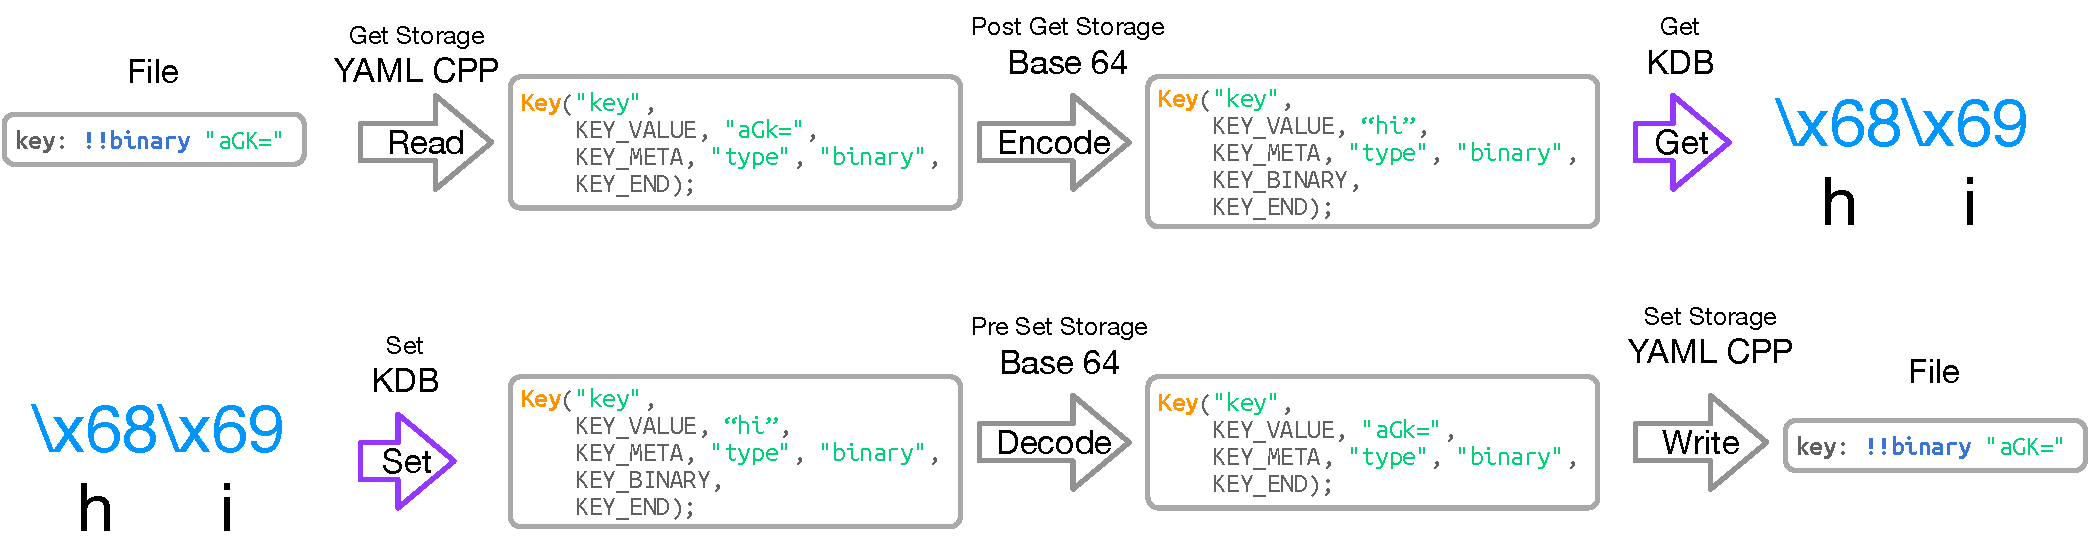
\includegraphics[width=\textwidth]{Base64}
  \caption{The Base64 plugin decodes and encodes binary data}
  \label{fig:base64}
\end{figure}

\subsection{Directory Value}

We already described the problem of storing a value in a non-leaf (directory) \cc{Key} in the Section~“\nameref{sec:mapping_elektra_yaml}”. Since the problem is independent of the parser engine and also relevant to other plugins, we implemented the functionality in a plugin named \href{http://libelektra.org/plugins/directoryvalue}{Directory Value}.

The Directory Value plugin adds an additional \cc{Key} with the prefix \yaml{___dirdata} for every non-array \cc{Key} that has children and contains a value in the \code{set} direction (position \code{preset}). For example, for the \cc{KeySet} shown in Figure~\ref{fig:keyset_large}, the plugin adds the \cc{Key}

\begin{itemize}
  \item \code{user/yaml/bloc/\_\_\_dirdata} and
  \item \code{user/yaml/bloc/party/\_\_\_dirdata}
\end{itemize}

. The plugin then moves the data stored in the parent \cc{Key} to the newly created \cc{Key}.

\begin{figure}[H]
  \centering
  \begin{subfigure}[t]{.4\textwidth}
    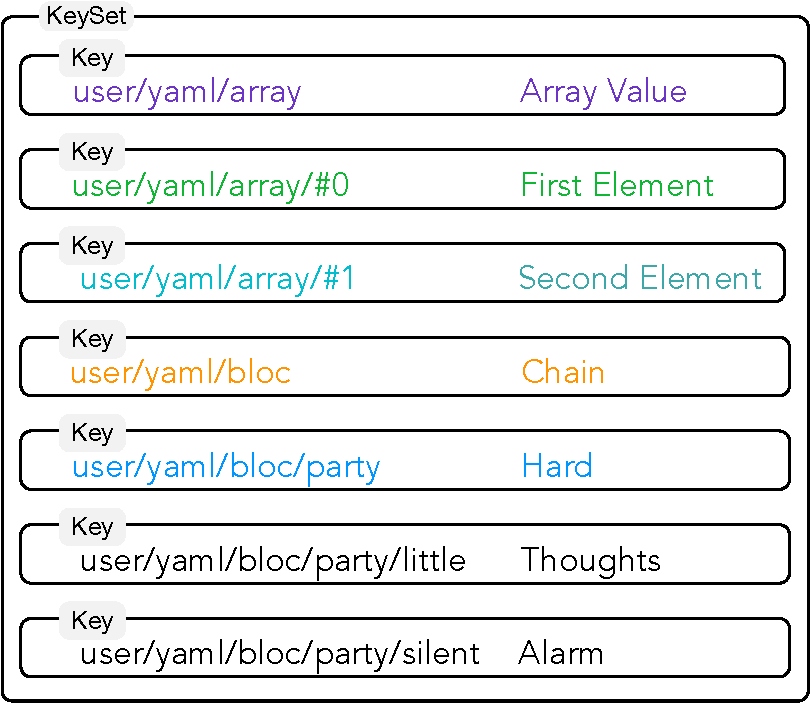
\includegraphics[width=\linewidth]{KeySetLarge}
    \caption{We use the \cc{KeySet} above as input for the Directory Value plugin at the \code{preset} position.}
    \label{fig:keyset_large}
  \end{subfigure}
  \qquad
  \begin{subfigure}[t]{.48\textwidth}
    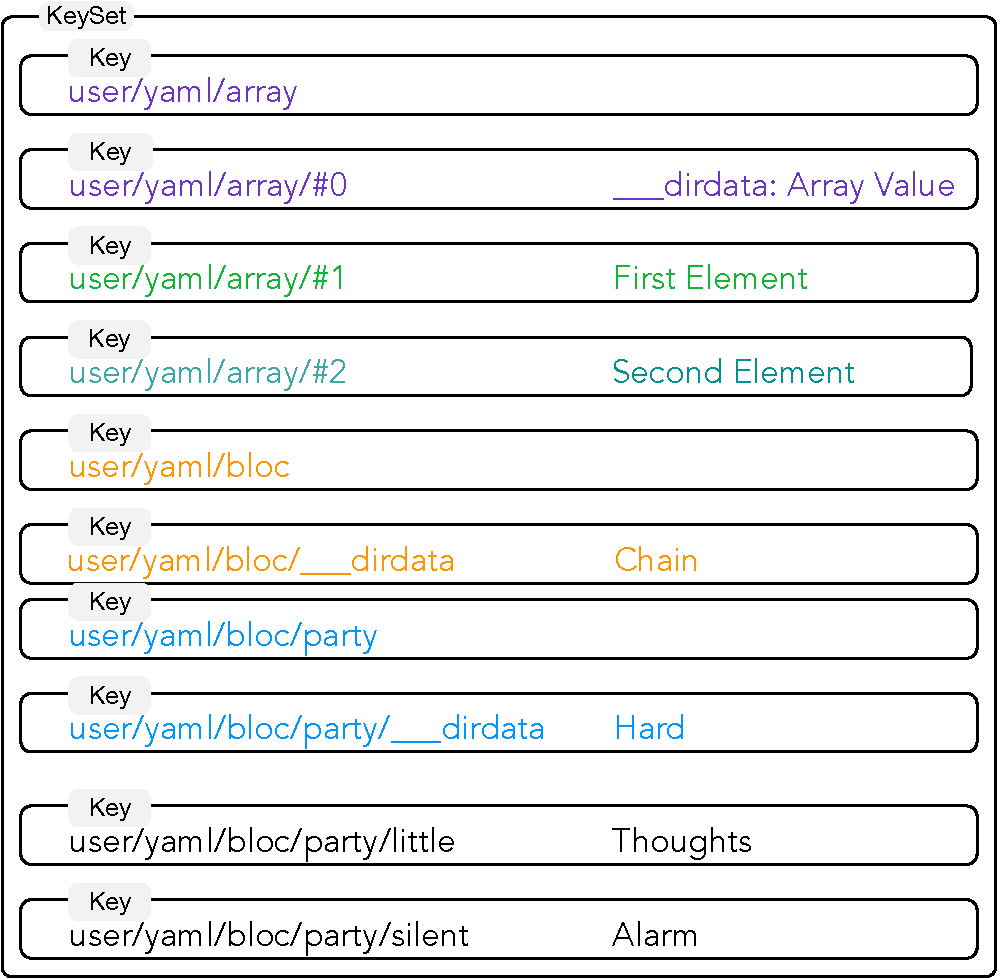
\includegraphics[width=\linewidth]{KeySetLargeExtended}
    \caption{The \cc{KeySet} above shows the result of the conversion at the \code{preset} position.}
    \label{fig:keyset_large_extended}
  \end{subfigure}
  \caption{The Directory Value plugin adds data at the position \code{preset} (\ref{fig:keyset_large_extended}) and then restores the original data (\ref{fig:keyset_large}) at the position \code{postget}.}
\end{figure}

In addition the plugin insert a new \cc{Key} for every array parent that stores a (non-binary) value, at the first position of the array. In our example, the plugin adds a new \cc{Key} with the value \code{\_\_\_dirdata: Array Value} at the first position of \code{user/yaml/array}, and increases the index of all other array elements by one.

Figure~\ref{fig:keyset_large_extended} shows the \cc{KeySet} after the whole conversion at the position \code{preset}. This \cc{KeySet} is also the input for the Directory Value plugin at the position \code{postget}.

\subsection{\glstext{YAML} Smith}

Elektra’s storage plugins need to both

\begin{enumerate}
  \item convert a configuration file to a \cc{KeySet}, and
  \item convert a \cc{KeySet} to a configuration file
\end{enumerate}

. Since the second task is always the same, regardless of the parser library we use, we created a plugin called \href{http://libelektra.org/plugins/yamlsmith}{YAML Smith} that takes care of this task.
